\scanpage{37}\mspage{$\underline{\overline{\mathrm{X}}}$}
% P1; upper pencil objection and its detached diagonal leader.
\margin{!!}Reste le cas $\mathring{T}\cap\Gamma\ne\unsure{\phi|\varnothing}$. Considerons l'enveloppe convexe\margin{\begin{tikzpicture}[x=1mm,y=1mm,baseline]\draw (0,0)--(6,8);\end{tikzpicture}\quad ce n'est \unsure{pas une|pas un} ``\unsure{env. conv.|ens. conv.}''!} $\unsure{\mathbb{C}|C}$ de $(\mathring{T}\cup\inserted{\bigl[}]s',s''[\inserted{\bigr]})\cap\Gamma$.

% P2
On a $\mathbb{C}\subset T-([s,s']\cup[s,s''])$. Observons que $S(\partial C)\deleted{\unsure{\subset|\cap}}\cap\mathring{T}\subset S(\Gamma)$.

% P3; the detached apostrophe between il and y is visible.
Comme $\mathring{T}\cap\Gamma\ne\phi$ il'y a\deleted{\illegible{1}} au moins un sommet de $\partial C$ à l'interieur $\mathring{T}$. \unsure{Le|le} lemme $\underline{\overline{\mathrm{IV}}}$ montre qu'il existe $y\notin S(\partial C)$, $y\in\mathbb{C}$, tel que $y$ est $(\mathbb{R}^2-\mathbb{C})$-visible de $s$

% P4
(Noter aussi que $\mathring{C}\ne\phi$ puisque $\Gamma\cap\mathring{T}\ne\phi\Rightarrow\operatorname{card}(\Gamma\cap]s',s''[)\geq 2$)

% P5
Soit $\alpha\in A(\partial C)$ telle que $y\in\alpha$ le lemme V montre que tout point de $\alpha$ est $(\mathbb{R}^2-C)$-visible de $s$. Si $\alpha=[z,z']$ montrons que $z^{\deleted{\unsure{\prime}}}\notin[s',s'']$ ou bien $z^{\unsure{\prime|\prime\prime}}\notin[s',s'']$. Soit donc $z''\in\mathring{T}\cap\Gamma$ et considerons le triangle $T'$ de sommets $z,z',z''$. Si $z',z''\in[s',s'']$ on voit que $]\unsure{s|S},y[$ ($y\in]z,z'[$) coupe $\mathring{T}'$ selon un ensemble non-vide. Cela contredit le choix de $y$ puisque $\mathring{T}'\subset\mathbb{C}$, \deleted{\unsure{C.a|c.a|c.à}} donc $z'$ par exemple vérifie $z'\notin[s',s'']$, $z'\in S'(\Gamma)$ (puisque $z'\in S(\partial\mathbb{C})\cap\mathring{T}$) et le lemme \deleted{\unsure{3|5}} V montre que $z'$ est $(\mathbb{R}^2-\mathbb{C})$-visible de $s$, donc $\operatorname{int}\Gamma$-visible de $s$, c.q-f.d.
% Long left-margin pencil note, written sideways and in staggered short groups.
% Its long curved pencil rule begins beside On a and continues beside the note.
\margin{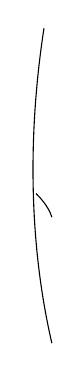
\begin{tikzpicture}[x=1mm,y=1mm]\draw (1,40)..controls (-1,27) and (-1,13)..(2,0);\draw (0,19)..controls (1,18) and (1.7,17)..(2,16);\end{tikzpicture}\par compliqué, prendre un sommet de $\Gamma$ $\in$ \deleted{\unsure{$\mathring T$|$\alpha$}} et qui est à dist. max. de la droite \deleted{\unsure{$\Delta$}} $(s's'')$}

% P6: pencil underline and exclamation marks.
\uline{Corollaire à la demonstration du lemme $\underline{\overline{\mathrm{VIII}}}$.} \margin{!!}

% P7: pencil word and its curved insertion leader.
Si $\Gamma$ est un polygone il existe un couple de sommets \inserted{\unsure{distincts}}\margin{\begin{tikzpicture}[x=1mm,y=1mm]\draw (0,0)..controls (-1,4) and (4,4)..(8,5)..controls (12,6) and (15,6)..(16,8);\end{tikzpicture}} $s,s'\in S(\Gamma)$ tels que $s'$ est \deleted{vis} $(\mathbb{R}^2-\Gamma)$-visible de $s$ et $]s',s[\subset\partial E(\Gamma)$.
% archive sheet number: 36
